\documentclass[border=10pt]{standalone}

\usepackage{tikz}
\usepackage{tikzsymbols}
\usetikzlibrary{calc,patterns,shapes.geometric}

\def\centerarc[#1](#2)(#3:#4:#5){\draw[#1] ($(#2)+({#5*cos(#3)},{#5*sin(#3)})$) arc (#3:#4:#5);}

\begin{document}
	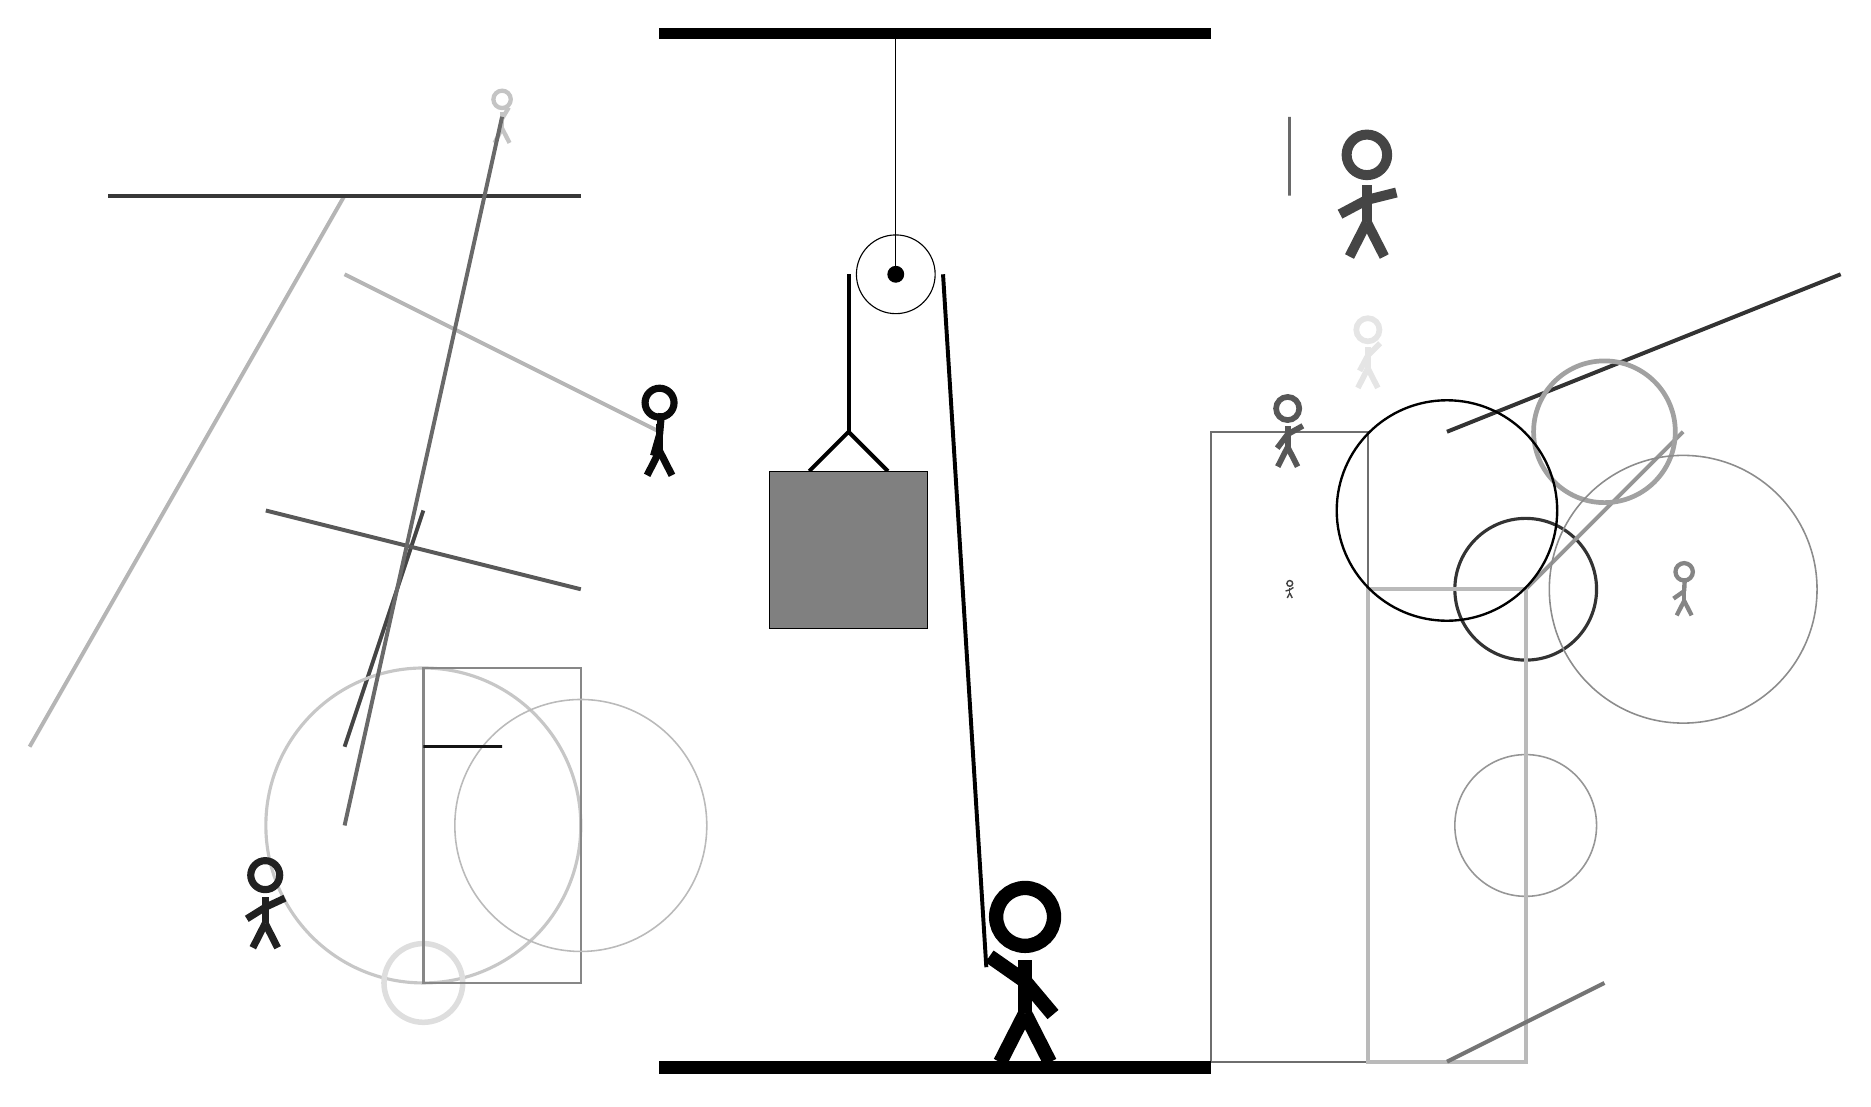
\begin{tikzpicture}
		%%%%% START %%%%%
		
		\draw[fill=black] (-2, 10) rectangle (5, 10.125);
		
		\draw (1, 7) circle (0.5);
		\draw[fill=black] (1, 7) circle (0.1);
		\draw (1, 10) -- (1, 7);
		
		\draw[line width=0.5mm] (-0.1, 4.5) -- (0.4, 5.0) -- (0.9, 4.5);
		\draw[fill=black!50] (-0.6, 4.5) rectangle (1.4, 2.5);
		
		\draw[line width=0.5mm, color=black!29](-2, 5) -- (-6, 7);
		
		\draw [line width=0.4mm, color=black!80](9, 3) circle (0.9);
		\node[line width=0.5mm, color=black!23] at (-4, 9) {\Strichmaxerl[3][79][59]};
		\draw[line width=0.5mm, color=black!73](-6, 1) -- (-5, 4);
		\draw [line width=0.4mm, color=black!22](-5, 0) circle (2.0);
		
		\node[line width=0.6mm, color=black!10] at (7, 6) {\Strichmaxerl[4][62][45]};
		\draw [line width=0.7mm, color=black!13](-5, -2) circle (0.5);
		\draw [line width=0.2mm, color=black!41](9, 0) circle (0.9);
		\node[line width=0.5mm, color=black!96] at (-2, 5) {\Strichmaxerl[5][74][85]};
		
		\node[line width=0.6mm, color=black!74] at (6, 3) {\Strichmaxerl[1][15][34]};
		\draw[line width=0.5mm, color=black!41](9, 3) -- (11, 5);
		\draw[line width=0.3mm, color=black!47] (-3, -2) rectangle (-5, 2);
		\draw[line width=0.5mm, color=black!65](-7, 4) -- (-3, 3);
		\draw [line width=0.2mm, color=black!27](-3, 0) circle (1.6);
		\draw[line width=0.3mm, color=black!57] (5, 5) rectangle (7, -3);
		\draw[line width=0.5mm, color=black!59] (6, 8) rectangle (6, 9);
		\draw[line width=0.5mm, color=black!80](8, 5) -- (13, 7);
		\draw[line width=0.5mm, color=black!29](-6, 8) -- (-10, 1);
		\node[line width=0.5mm, color=black!48] at (11, 3) {\Strichmaxerl[3][35][87]};
		
		\draw[line width=0.5mm, color=black!78](-3, 8) -- (-9, 8);
		\node[line width=0.5mm, color=black!87] at (-7, -1) {\Strichmaxerl[5][32][25]};
		
		\draw[line width=0.5mm, color=black!27] (7, 3) rectangle (9, -3);
		\draw [line width=0.6mm, color=black!37](10, 5) circle (0.9);
		\node[line width=0.6mm, color=black!66] at (6, 5) {\Strichmaxerl[4][53][29]};
		\node[line width=0.5mm, color=black!73] at (7, 8) {\Strichmaxerl[7][28][14]};
		
		\draw [line width=0.3mm, color=black!100](8, 4) circle (1.4);
		\draw[line width=0.4mm, color=black!92] (-4, 1) rectangle (-5, 1);
		\draw [line width=0.2mm, color=black!45](11, 3) circle (1.7);
		
		\draw[line width=0.5mm, color=black!54](10, -2) -- (8, -3);
		\draw[line width=0.5mm, color=black!59](-4, 9) -- (-6, 0);
		
		\draw[line width=0.5mm] (0.4, 7) -- (0.4, 5.0);
		\centerarc[line width=0.5mm](1, 7)(0:180:0.6);
		\draw[line width=0.5mm](1.6, 7) -- (2.15, -1.8);
		
		\node at (2.6, -1.9) {\Strichmaxerl[10][-35][-50]};
		
		\draw[fill=black] (-2, -3) rectangle (5, -3.15);
		
		%%%%% END %%%%%
	\end{tikzpicture}
\end{document}